\documentclass[a4paper,12pt]{report}

\usepackage{cmap}
\usepackage[T2A]{fontenc}
\usepackage[utf8]{inputenc}
\usepackage[english,russian]{babel}
\usepackage{listings}
\usepackage{amsmath}
\usepackage{amsfonts}
\usepackage{float}
\usepackage{csquotes}
\usepackage{hyphenat}

% \usepackage{titlesec}
% \newcommand{\sectionbreak}{\clearpage}

\usepackage{graphicx}
\graphicspath{ {./images/} }

\usepackage{xcolor}
% \usepackage{courier}

\usepackage[
    backend=biber,
    style=alphabetic,
    sorting=ynt
]{biblatex}
\addbibresource{resources.bib}

\definecolor{buzzlightyear}{HTML}{8757A5}
\definecolor{grass}{HTML}{738D06}
\definecolor{sand}{HTML}{F18A2B}
\definecolor{comment}{HTML}{8E908B}

\lstdefinestyle{habrstyle}{
    backgroundcolor=\color{white},   
    commentstyle=\color{comment},
    keywordstyle=\bfseries\color{buzzlightyear},
    numberstyle=\tiny\color{comment},
    stringstyle=\color{grass},
    basicstyle=\ttfamily\footnotesize,
    breakatwhitespace=false,         
    breaklines=true,                 
    captionpos=b,                    
    keepspaces=true,                 
    numbers=left,                    
    numbersep=5pt,                  
    showspaces=false,                
    showstringspaces=false,
    showtabs=false,                  
    tabsize=4
}

\lstset{style=habrstyle}

\author{Луняк Николай}
\title{Лабораторная работа 12}
\date{\today}

\begin{document}
    \maketitle
    \tableofcontents
    \listoffigures
    \lstlistoflistings
    
    \chapter{Общее}
    \section{Цели}
    
    Суть данной работы заключается в том, чтобы:
    
    \begin{itemize}
        \item получить представление о проблемах искажения сигналов и \textquote{канальных эффектах}
        
        \item определять стадии, необходимые для восстановления сигналов:
        \begin{itemize}
            \item временное восстановление
            \item многопутевые каналы
            \item коррекция фазы и частоты
            \item декодирование символов и порядок бит
        \end{itemize}
    \end{itemize}
    
    \section{Окружение}
    
    Так как официально Windows не поддерживается, буду работать на Arch. Вроде бы достаточно только установить \texttt{gnuradio} и все... а нет, говорит:
    
    \begin{figure}[H]
        \centering
        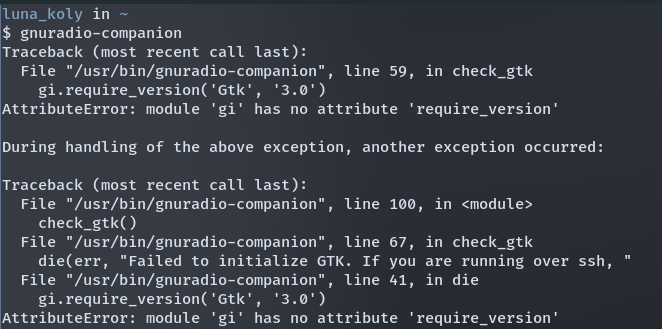
\includegraphics[width=0.75\textwidth]{images/error_1.png}
        \caption{Проблема 1}
        \label{fig:error_1}
    \end{figure}
    
    В интернетах пишут, нужно установить \texttt{python-gobject}. Пробуем.
    
    \begin{figure}[H]
        \centering
        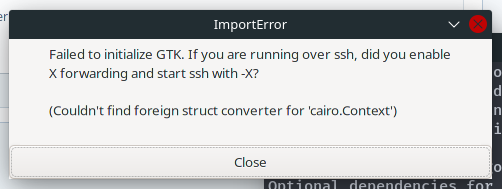
\includegraphics[width=0.75\textwidth]{images/error_2.png}
        \caption{Проблема 2}
        \label{fig:error_2}
    \end{figure}
    
    Классное ПО.
    
    О, я не одинок: https://bbs.archlinux.org/viewtopic.php?id=252150. Что ж, перезапустим... неа, то же самое.
    
    В консоли написано: \textquote{Gtk-Message: 14:22:04.664: Failed to load module "appmenu-gtk-module"}. Установим. Все равно та же картинка, только теперь еще и в консоли нет никаких сообщений. Классное ПО.
    
    Попробуем установить еще и \texttt{python-cairo}.
    
    Ура, что-то открылось:
    
    \begin{figure}[H]
        \centering
        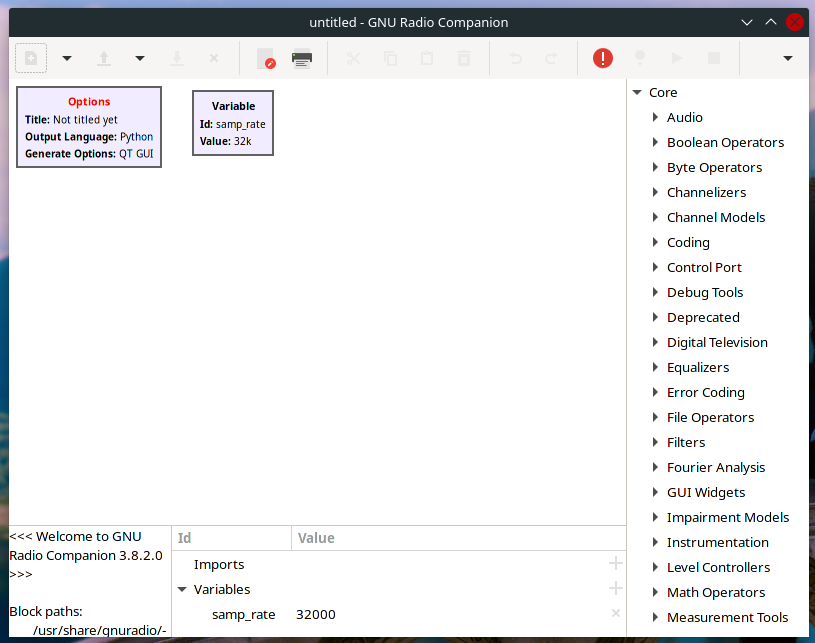
\includegraphics[width=0.75\textwidth]{images/window.png}
        \caption{Что-то}
        \label{fig:window}
    \end{figure}
    
    Попробовал сделать простейший граф, а получил это:
    
    \begin{figure}[H]
        \centering
        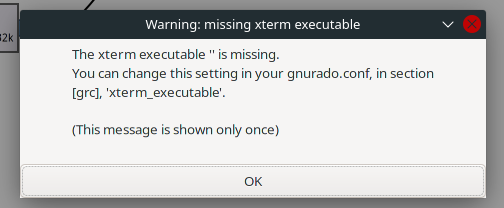
\includegraphics[width=0.75\textwidth]{images/error_3.png}
        \caption{Опять}
        \label{fig:error_3}
    \end{figure}
    
    Какого дьявола я обязан устанавливать \texttt{xterm}, я совершенно не понимаю, это абсурд.
    
    Мало этого,
    
    \begin{figure}[H]
        \centering
        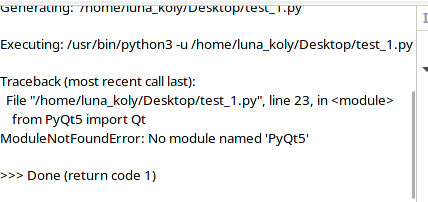
\includegraphics[width=0.75\textwidth]{images/error_4.png}
        \caption{Опять}
        \label{fig:error_4}
    \end{figure}
    
    Выбора нет, придется все это ставить. Если что, я не случайно пользуюсь Arch'ем, у меня места осталось 1ГБ, и если оно закончится, я буду \emph{очень} расстроен.
    
\begin{lstlisting}[caption=Опять какая-то фигня]
Executing: /usr/bin/python3 -u /home/luna_koly/Desktop/test_1.py

Traceback (most recent call last):
  File "/usr/lib/python3.9/site-packages/gnuradio/qtgui/__init__.py", line 32, in <module>
    from .qtgui_swig import *
  File "/usr/lib/python3.9/site-packages/gnuradio/qtgui/qtgui_swig.py", line 13, in <module>
    from . import _qtgui_swig
ImportError: libqwt.so.6: cannot open shared object file: No such file or directory

During handling of the above exception, another exception occurred:

Traceback (most recent call last):
  File "/home/luna_koly/Desktop/test_1.py", line 24, in <module>
    from gnuradio import qtgui
  File "/usr/lib/python3.9/site-packages/gnuradio/qtgui/__init__.py", line 36, in <module>
    from .qtgui_swig import *
  File "/usr/lib/python3.9/site-packages/gnuradio/qtgui/qtgui_swig.py", line 13, in <module>
    from . import _qtgui_swig
ImportError: libqwt.so.6: cannot open shared object file: No such file or directory

>>> Done (return code 1)
\end{lstlisting}
    
    Это просто сюр какой-то, это ну невозможно просто.
    
    Хорошо, сделаем так, как говорят тут: https://github.com/gnuradio/gnuradio/issues/3117, и установим еще и \texttt{qwt}.
    
    Вот теперь я получил какой-то график, наконец.
    
    Но нельзя просто так взять и запустить GNU Radio...
    
    \begin{figure}[H]
        \centering
        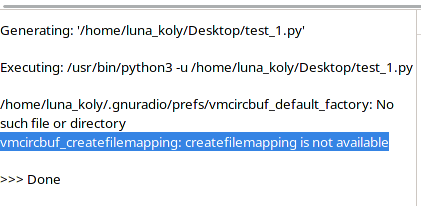
\includegraphics[width=0.75\textwidth]{images/error_5.png}
        \caption{Очередные бульканья GNU Radio}
        \label{fig:error_5}
    \end{figure}
    
    Ну и дьявол с ним!
    
    \chapter{Передача QPSK-сигнала}
    
    QPSK означает Quadrature Phase-Shift Keying\cite{qpsk_wiki}, что есть фазовая модуляция, подразумевающая использование 4 точек constellation diagram (двумерной плоскости, на которой комплексным числам будут соответствовать наши символы). 
    
    Для простой передачи сигнала нам потребуется модулятор (\sloppy{\texttt{Constellation Modulator Block}}) и \sloppy{\texttt{Constellaton Rect. Object}}, в который отвечает за то, как кодируются символы. Также нам потребуется генератор байтовых значений.
    
    Количество сэмплов на символ я оставлю тем же, что и в туториале (там этот выбор обосновывается наглядностью).
    
    Поэкспериментируем с выбором разной избыточной пропускной способности. Как я понимаю, этот параметр влияет на крутизну краев фильтра.
    
    \begin{figure}[H]
        \centering
        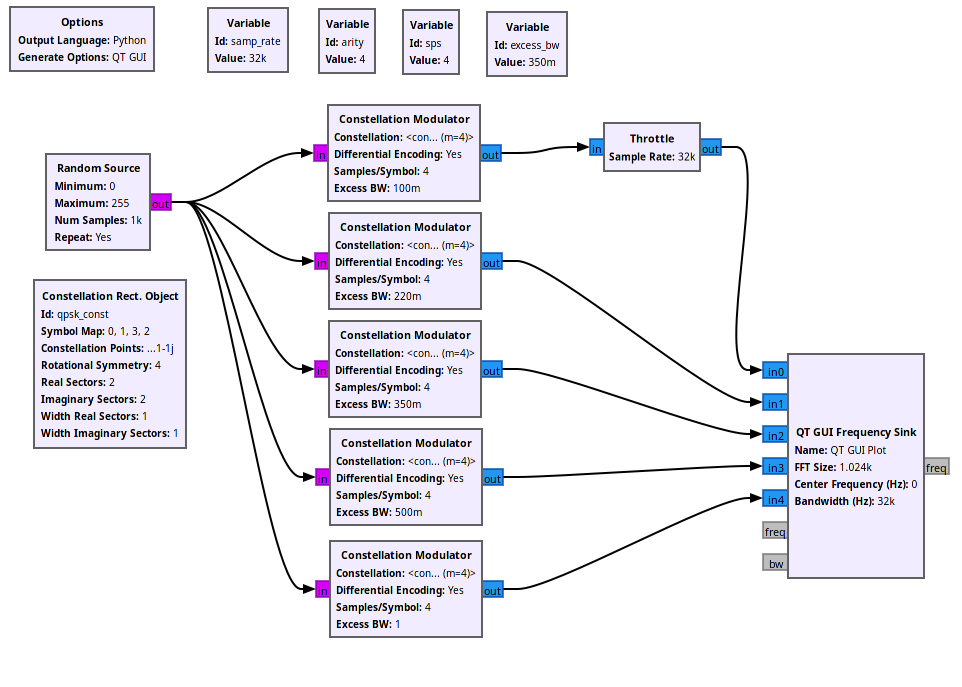
\includegraphics[width=0.75\textwidth]{images/mpsk_rrc_rolloff_fg.png}
        \caption{Flow Graph \texttt{mpsk\_rrc\_rolloff}}
        \label{fig:mpsk_rrc_rolloff_fg}
    \end{figure}
    
    И вот такой результат мы наблюдаем.
    
    \begin{figure}[H]
        \centering
        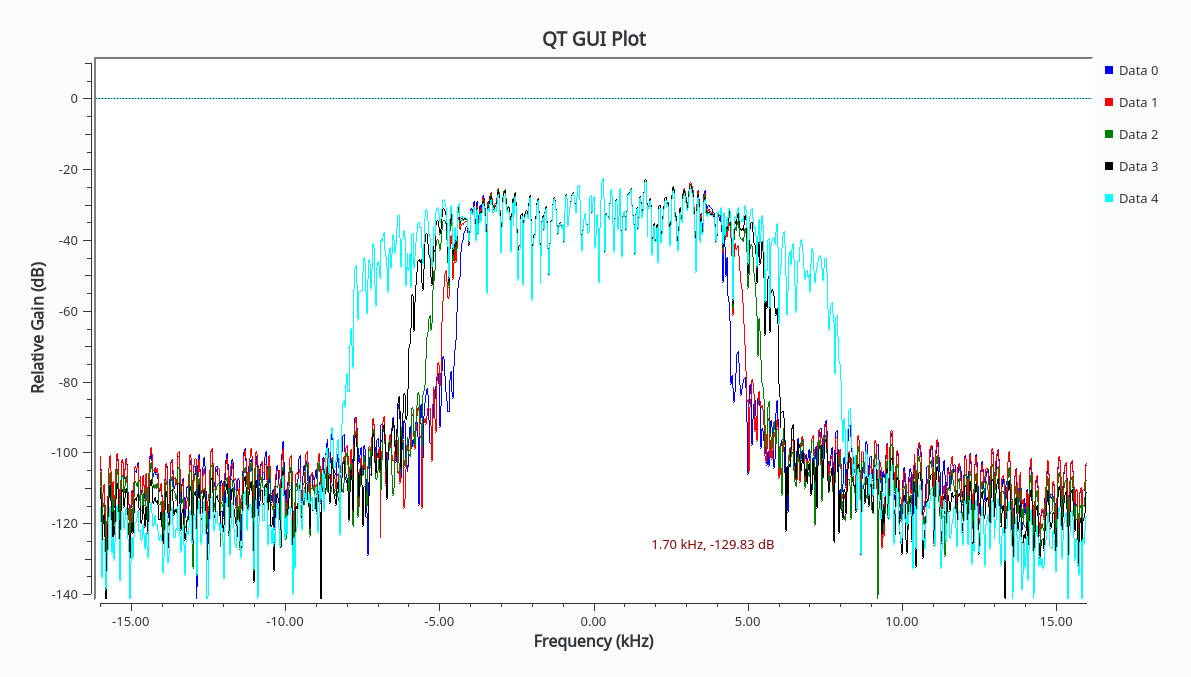
\includegraphics[width=0.75\textwidth]{images/mpsk_rrc_rolloff_plot.png}
        \caption{График \texttt{mpsk\_rrc\_rolloff}}
        \label{fig:mpsk_rrc_rolloff_plot}
    \end{figure}
    
    Чем больше excess bandwidth, тем более пологие края.
    
    Следующий Flow Graph осуществляет передачу QPSK-\textquote{созвездия} (честно, не знаю, насколько корректны мои попытки перевести термины на русский, поэтому дальше я буду использовать оба языка вперемешку, чтобы минимизировать путанницу). Он показывает переданный сигнал, полученный на приемнике сигнал во времени и частотах и созвездие.
    
    \begin{figure}[H]
        \centering
        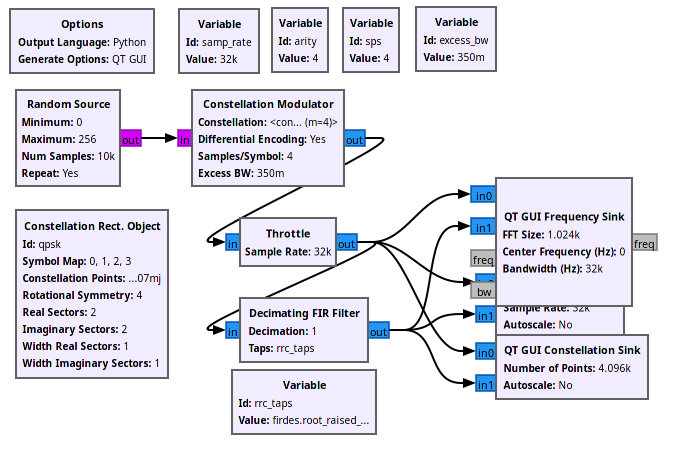
\includegraphics[width=0.75\textwidth]{images/mpsk_stage1_fg.png}
        \caption{Flow Graph \texttt{mpsk\_stage1}}
        \label{fig:mpsk_stage1_fg}
    \end{figure}
    
    \begin{figure}[H]
        \centering
        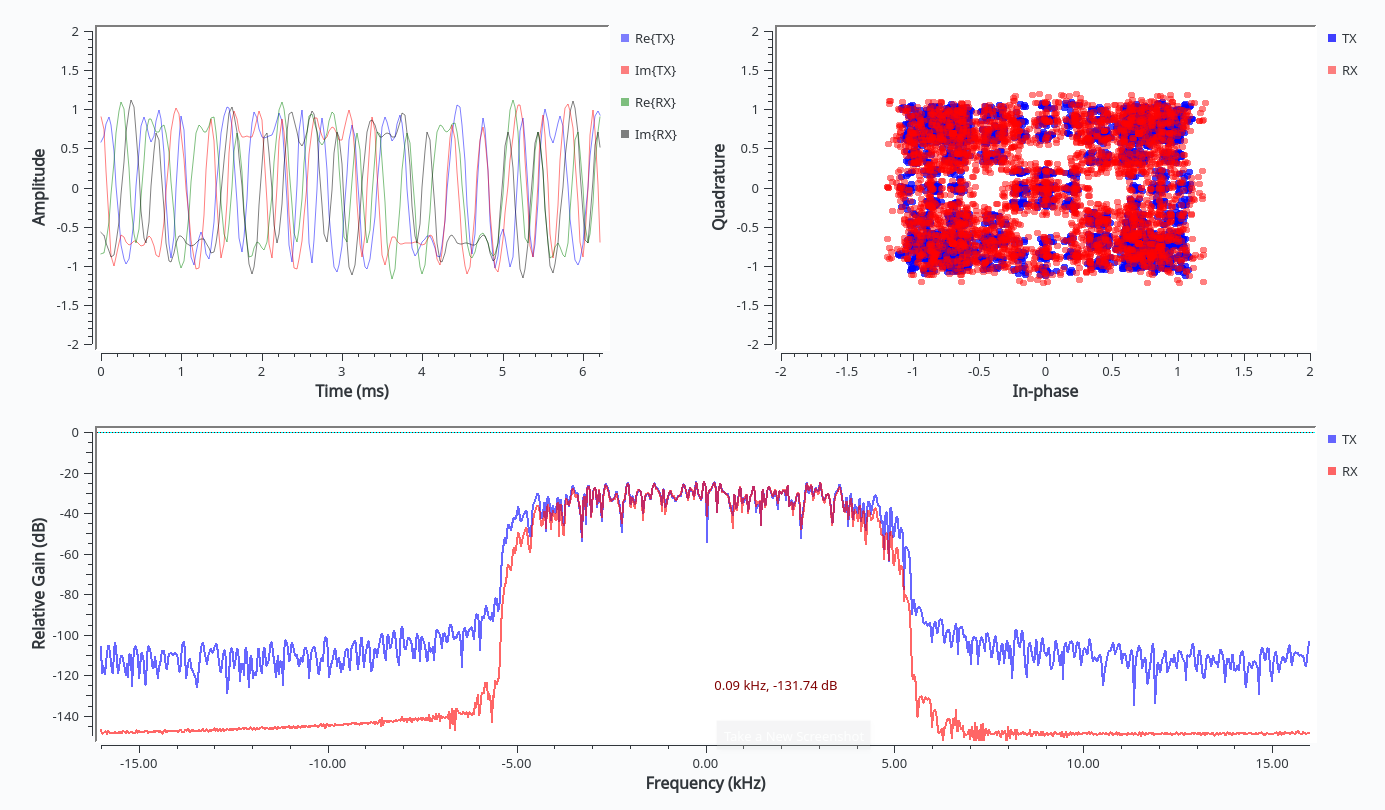
\includegraphics[width=0.75\textwidth]{images/mpsk_stage1_plot.png}
        \caption{График \texttt{mpsk\_stage1}}
        \label{fig:mpsk_stage1_plot}
    \end{figure}
    
    На созвездии можно видеть эффект увеличения частоты дискретизации (4 сэмпла на символ) и процесс фильтрации. В нашем случае RRC-фильтр специально добавляет помехи с самим собой (\textquote{межсимвольные помехи}) ISI. Это плохо для принятого сигнала, потому что тогда символы размываются.
    
    Чтобы избавиться от ISI мы на приемной стороне используем еще один RRC-фильтр. При помощи свертки мы получаем импульсы приподнятого косинуса с минимизированным ISI.
    
    \chapter{Искажения в канале}
    
    До этого мы рассматривали саму передачу сигнала, а теперь мы добавим искажения в канале перечач. Модель канала можно добавить при помощи \sloppy{\texttt{Channel Model}}.
    
    Канал позволит проиллюстрировать несколько проблем. Одна из них - шум. Мощность шума регулируется при помощи напряжения.
    
    Другая проблема - разные домены тактовых сигналов в приемнике и передатчике. Мало того, что может быть сдвиг, так еще и частоты не могут быть идеально точными, и потому содержат небольшую разницу.
    
    Третья проблема заключена в идеальной точке сэмплирования, которая не известна принимающей стороне.
    
    Flow Graph ниже позволяет манипулировать этими эффектами и наблюдать их влияние на сигнал:
    
    \begin{figure}[H]
        \centering
        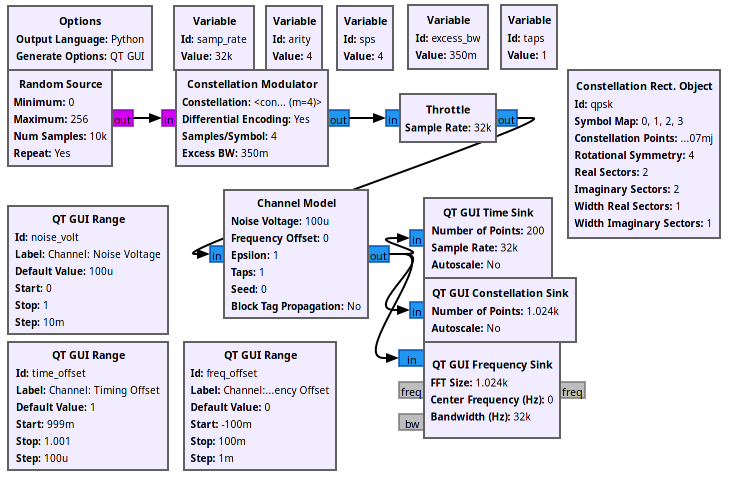
\includegraphics[width=0.75\textwidth]{images/mpsk_stage2_fg.png}
        \caption{Flow Graph \texttt{mpsk\_stage2}}
        \label{fig:mpsk_stage2_fg}
    \end{figure}
    
    И вот результат.
    
    \begin{figure}[H]
        \centering
        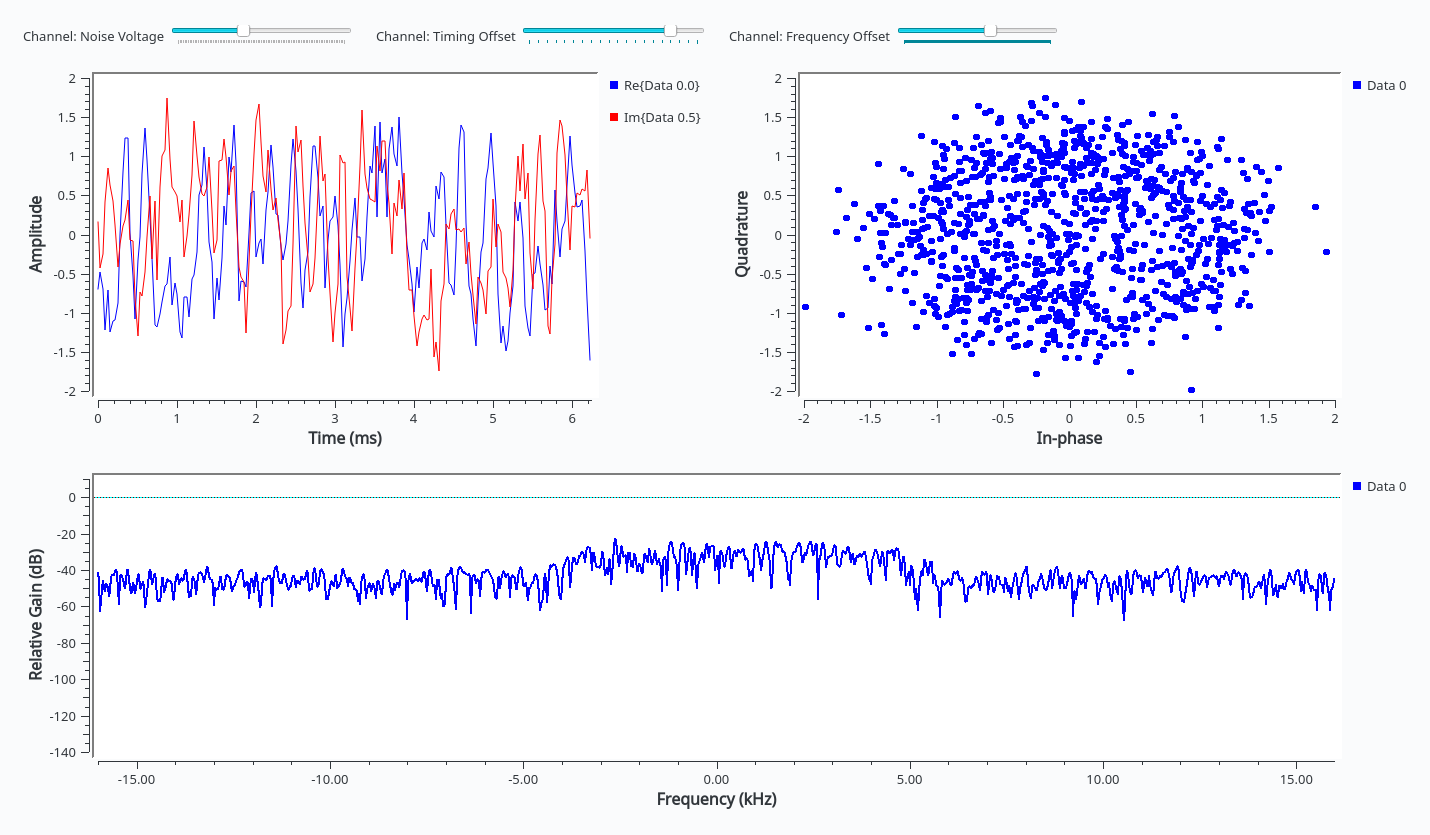
\includegraphics[width=0.75\textwidth]{images/mpsk_stage2_plot.png}
        \caption{График \texttt{mpsk\_stage2}}
        \label{fig:mpsk_stage2_plot}
    \end{figure}
    
    Видимо, насколько перемешанное получилось облако. Будем исправлять.
    
    \chapter{Временная коррекция}
    
    Вообще, есть много разных алгоритмов, некоторые даже могут произвести восстановление нескольких эффектов сразу, но мы воспользуемся алгоритмом полифазного восстановления тактового сигнала.
    
    Для восстановления времени, нам нужно отыскать наилучшее время для сэмплинга входящего сигнала, чтобы максимизировать SNR и минимизировать ISI.
    
    Следующий Flow Graph иллюстрирует проблему ISI, мы тут создаем 4 символа-единицы подряд, а затем фильтруем их:
    
    \begin{figure}[H]
        \centering
        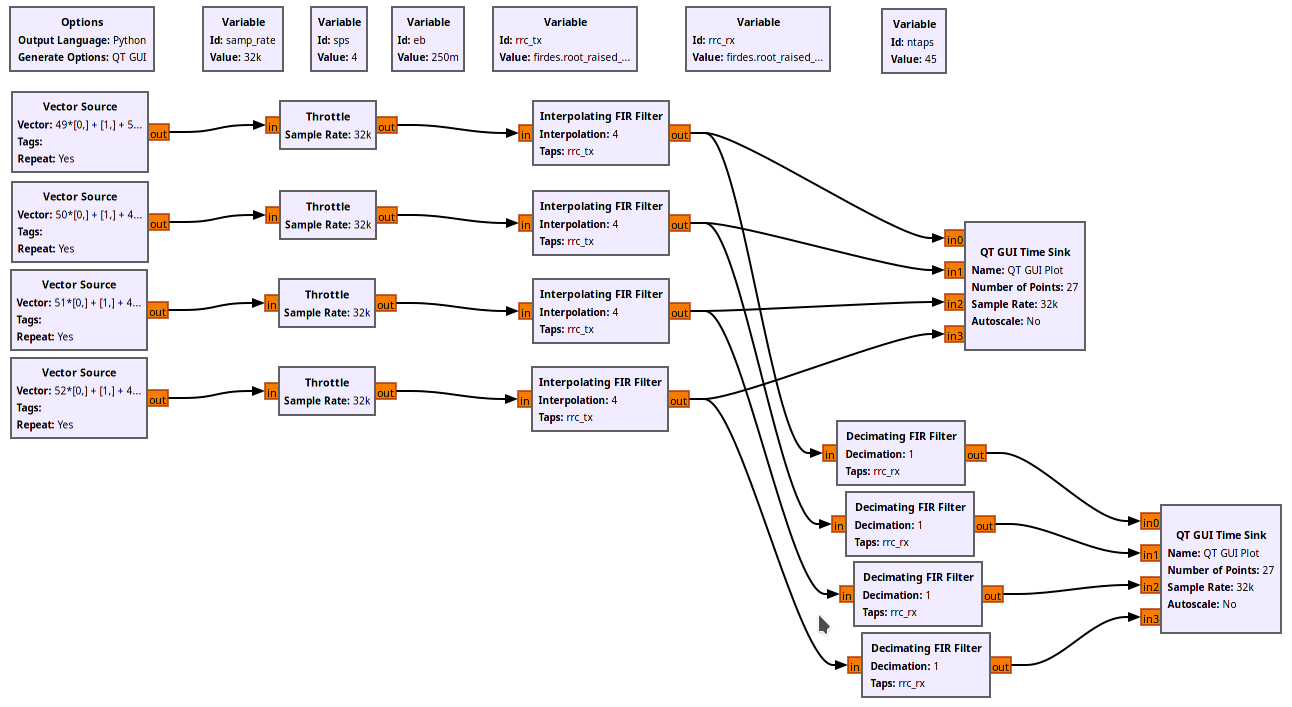
\includegraphics[width=0.75\textwidth]{images/symbol_sampling_fg.png}
        \caption{Flow Graph \texttt{symbol\_sampling}}
        \label{fig:symbol_sampling_fg}
    \end{figure}
    
    \begin{figure}[H]
        \centering
        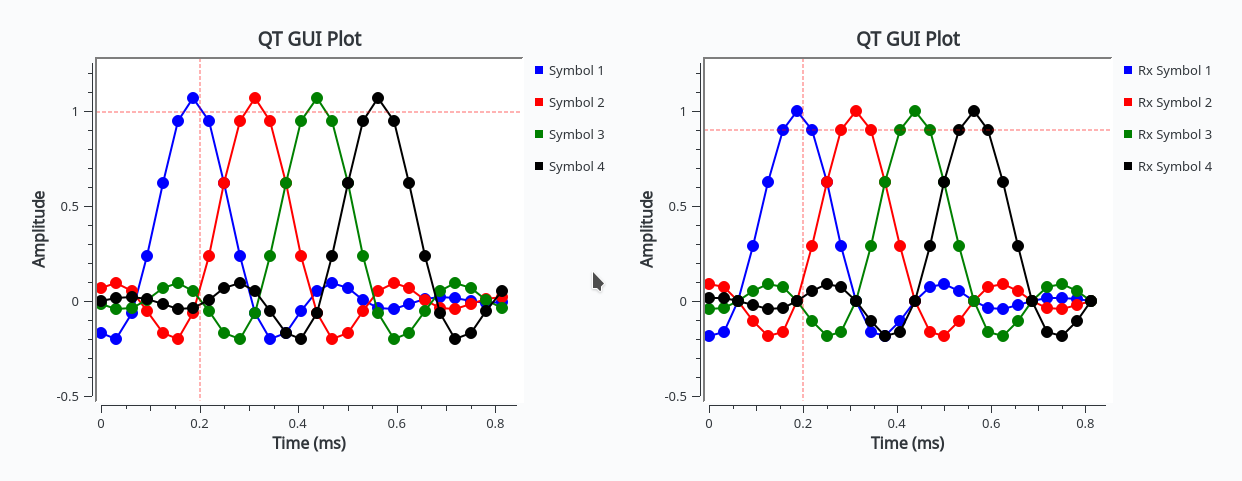
\includegraphics[width=0.75\textwidth]{images/symbol_sampling_plot.png}
        \caption{График \texttt{symbol\_sampling}}
        \label{fig:symbol_sampling_plot}
    \end{figure}
    
    Теперь посмотрим на эффект разных доменов тактовых сигналов на передатчике и приемнике. Разница во времени специально завышена для наглядности.
    
    \begin{figure}[H]
        \centering
        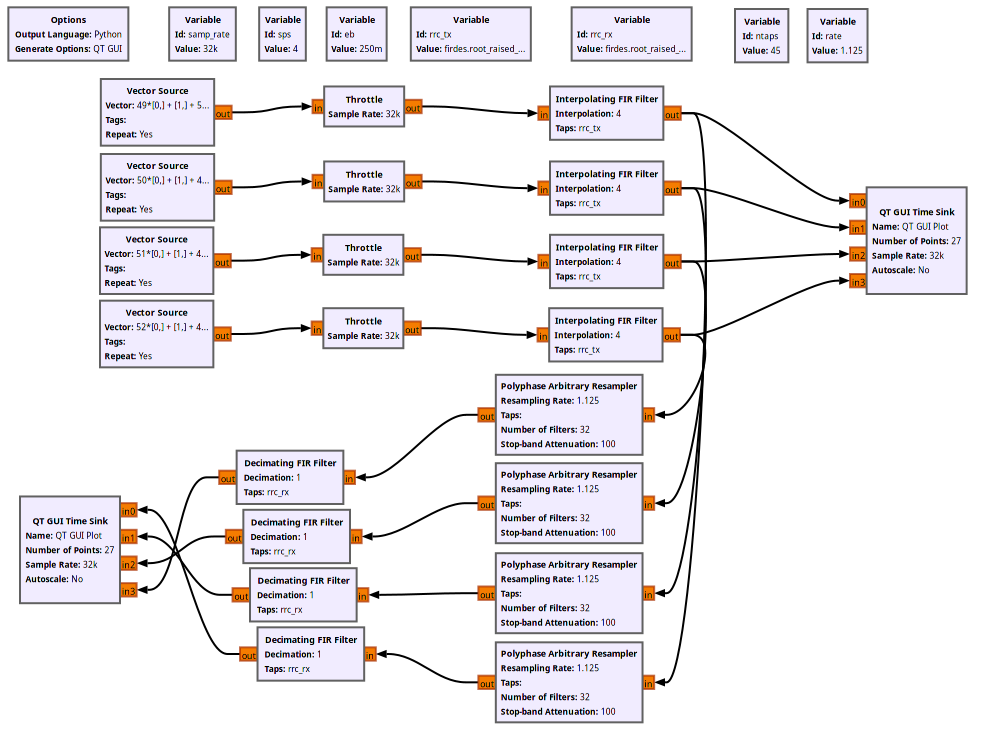
\includegraphics[width=0.75\textwidth]{images/symbol_sampling_diff_fg.png}
        \caption{Flow Graph \texttt{symbol\_sampling\_diff}}
        \label{fig:symbol_sampling_diff_fg}
    \end{figure}
    
    \begin{figure}[H]
        \centering
        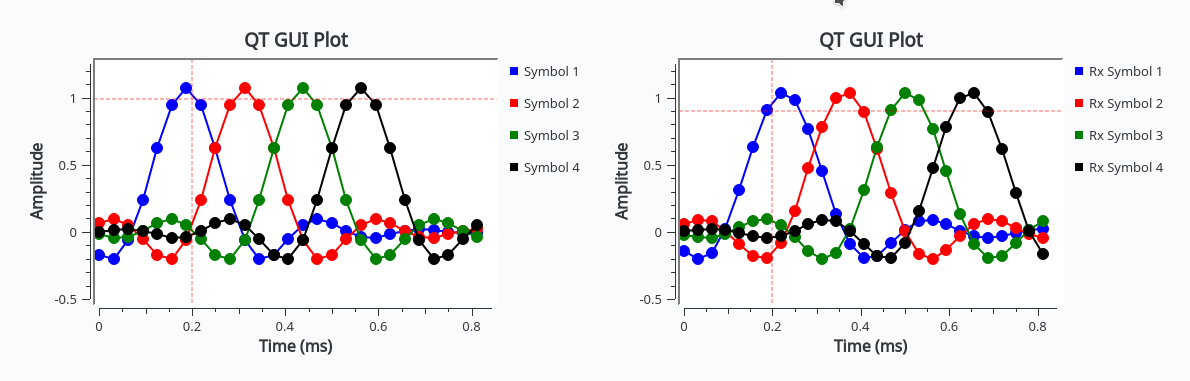
\includegraphics[width=0.75\textwidth]{images/symbol_sampling_diff_plot.png}
        \caption{График \texttt{symbol\_sampling\_diff}}
        \label{fig:symbol_sampling_diff_plot}
    \end{figure}
    
    Теперь нам надо синхронизировать все это дело.
    
    \section{Немного о блоке синхронизации многофазного тактового сигнала}
    
    Тут тоже много разных алгоритмов, но почти все они основаны на обратной связи (остальные получают в свое распоряжение дополнительную информацию). Мы сопользуеся техникой восстановления polyphase filterbank (кстати, она deprecated в GNU Radio 3.9). Она послужит для нескольких целей. Во-первых, она решит проблему с тактовыми доменами. Во-вторых, уменьшит ISI. В-третьих, понизит частоту дискретизации сигнала и будет производить по 1 сэмплу на символ.

    \begin{figure}[H]
        \centering
        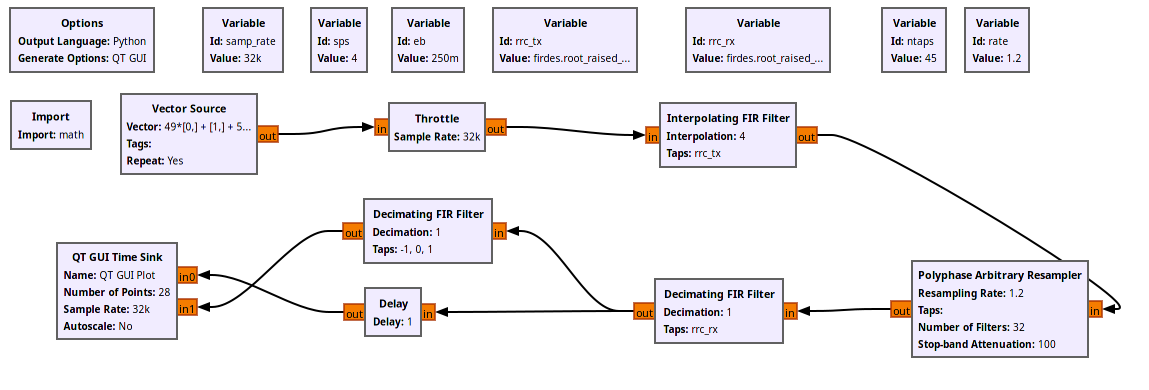
\includegraphics[width=0.75\textwidth]{images/symbol_differential_filter_fg.png}
        \caption{Flow Graph \texttt{symbol\_differential\_filter}}
        \label{fig:symbol_differential_filter_fg}
    \end{figure}
    
    \textquote{Идеальный} случай, где все хорошо и сдвига тактирующих сигналов нет должен был бы нам засечь значение в пике и нарисовать точку на графике производной при пересечении нуля, но из-за временного сдвига мы теперь ее не видим:
    
    \begin{figure}[H]
        \centering
        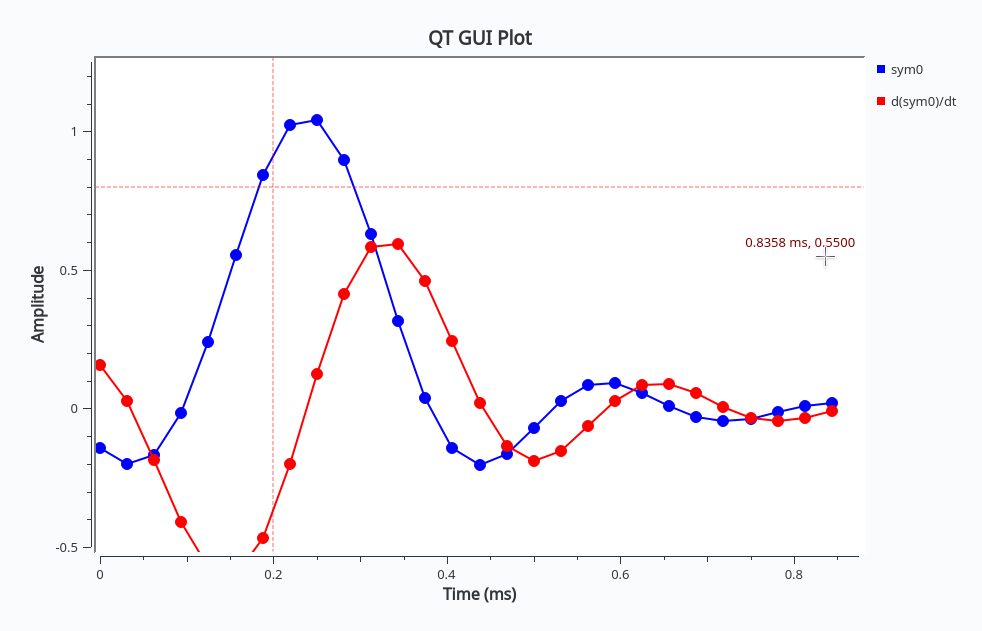
\includegraphics[width=0.75\textwidth]{images/symbol_differential_filter_plot.png}
        \caption{График \texttt{symbol\_differential\_filter}}
        \label{fig:symbol_differential_filter_plot}
    \end{figure}
    
    Можно попробовать использовать серию фильтров с разными сдвигами по фазам. Если их \emph{достаточно} много, можно надеяться, что какой-нибудь засечет правильную
    
    Тут пришлось вносить правки, потому что исходный Flow Graph был не доделан.
    
    \begin{figure}[H]
        \centering
        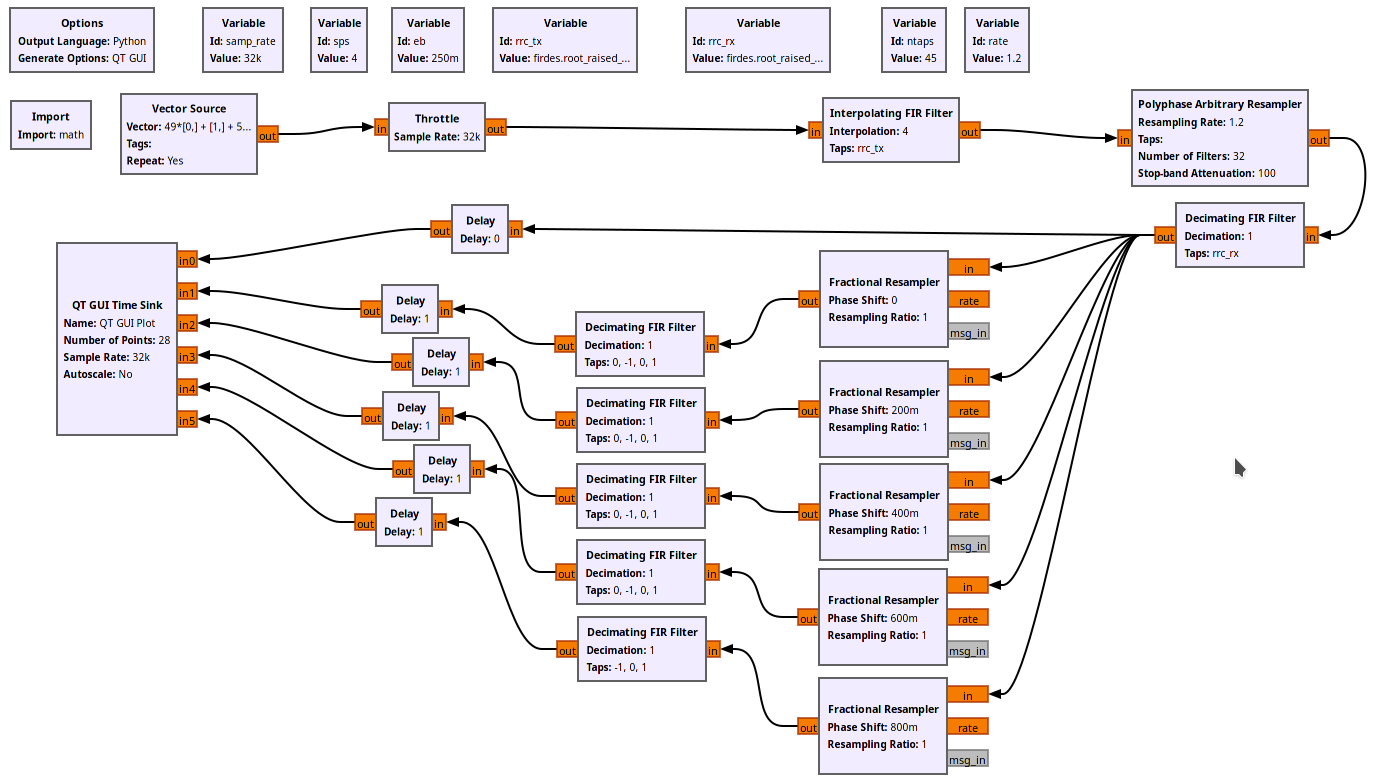
\includegraphics[width=0.75\textwidth]{images/symbol_differential_filter_phases_fg.png}
        \caption{Flow Graph \texttt{symbol\_differential\_filter\_phases}}
        \label{fig:symbol_differential_filter_phases_fg}
    \end{figure}
    
    \begin{figure}[H]
        \centering
        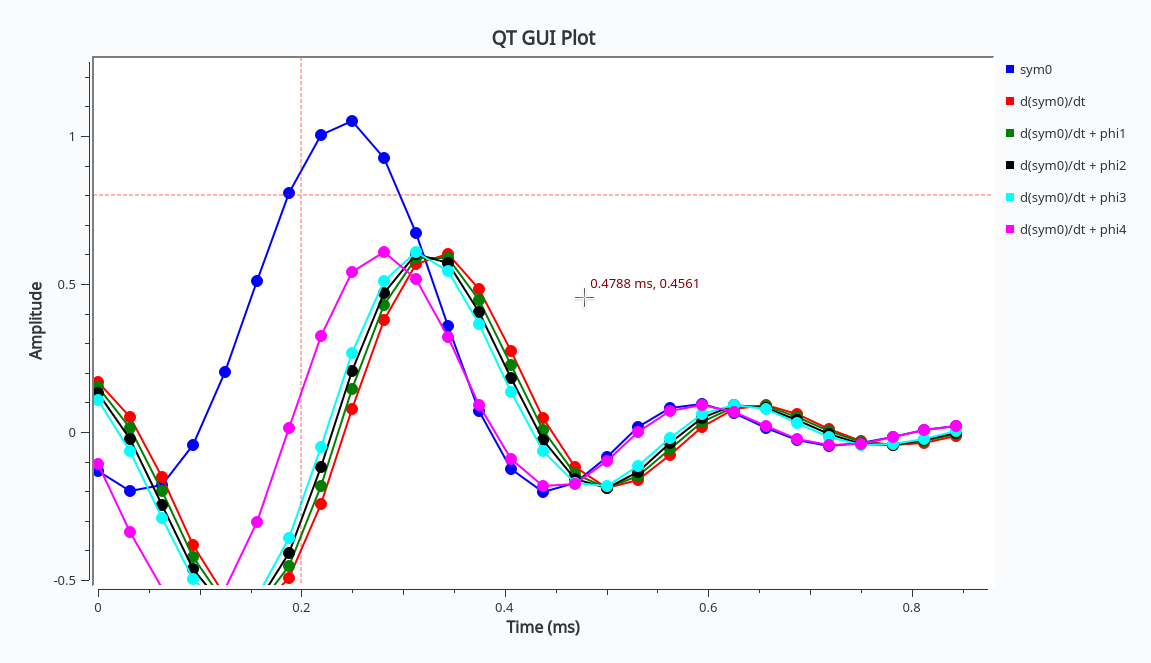
\includegraphics[width=0.75\textwidth]{images/symbol_differential_filter_phases_plot.png}
        \caption{График \texttt{symbol\_differential\_filter\_phases}}
        \label{fig:symbol_differential_filter_phases_plot}
    \end{figure}
    
    \section{Использование блока синхронизации полифазного тактирующего сигнала в нашем приемнике}
    
    Настроим блок на использование 32 фильтров:
    
    \begin{figure}[H]
        \centering
        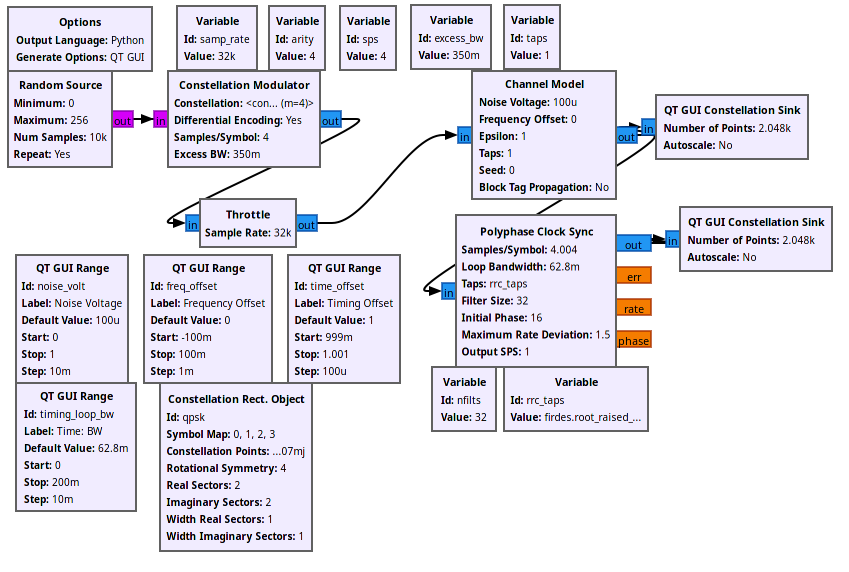
\includegraphics[width=0.75\textwidth]{images/mpsk_stage3_fg.png}
        \caption{Flow Graph \texttt{mpsk\_stage3}}
        \label{fig:mpsk_stage3_fg}
    \end{figure}
    
    И вот такой результат мы наблюдаем.
    
    \begin{figure}[H]
        \centering
        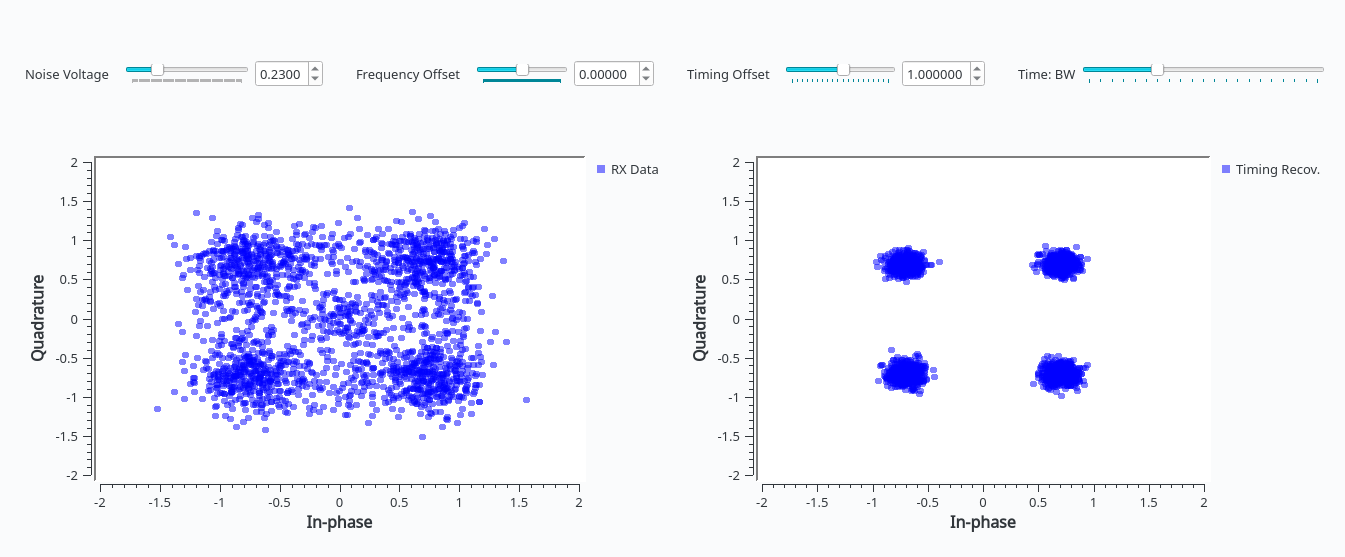
\includegraphics[width=0.75\textwidth]{images/mpsk_stage3_plot.png}
        \caption{График \texttt{mpsk\_stage3}}
        \label{fig:mpsk_stage3_plot}
    \end{figure}
    
    Вот они слева направо: полученный сигнал \textquote{до} восстановления времени и \textquote{после}.
    
    Если подвигать ползунок Timing Offset, то разница особо не заметна, а вот Frequency Offset сразу размазывает точки по всей окружности. Причем окружность еще и утолщается, что говорит и об ошибках в интрпретации абсолютных значений.
    
    \begin{figure}[H]
        \centering
        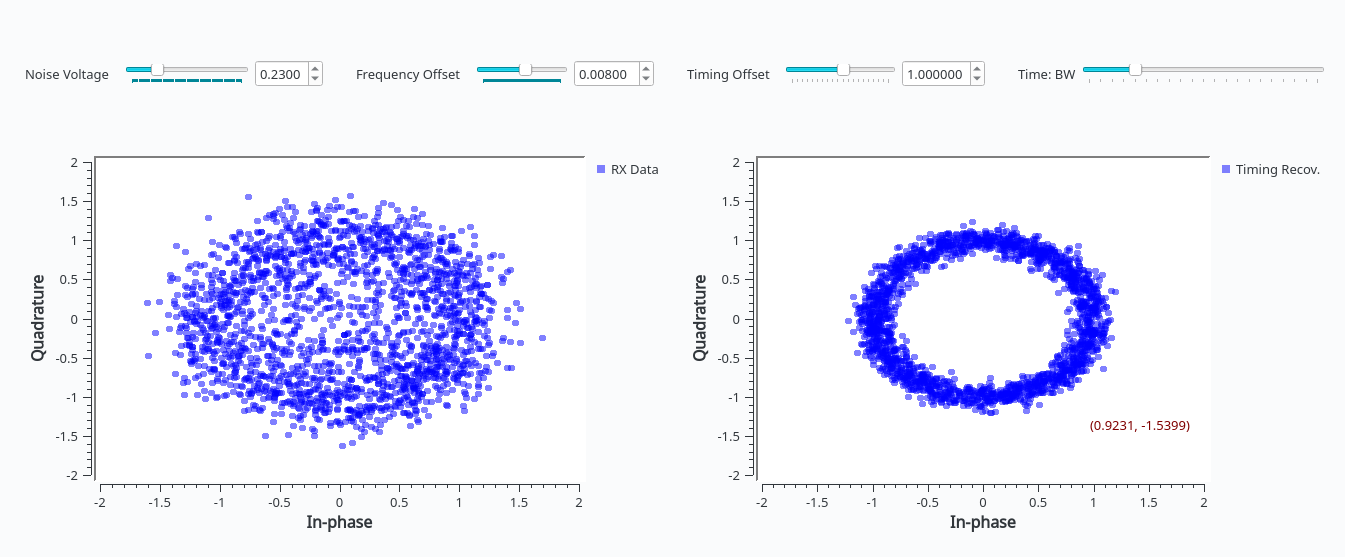
\includegraphics[width=0.75\textwidth]{images/mpsk_stage3_plot_freq.png}
        \caption{График \texttt{mpsk\_stage3} x2}
        \label{fig:mpsk_stage3_plot_freq}
    \end{figure}
    
    \chapter{Множество путей}
    
    Тут смысл в том, что обычно наш сигнал поступает на приемник с множества направлений сразу, что может приводить к искажениям.
    
    Чтобы справиться с искажениями, можно воспользоваться приемом, схожим со стерео-эквалайзерами. Как это выглядит в пространстве частот, можно видеть при помощи схемы ниже:
    
    \begin{figure}[H]
        \centering
        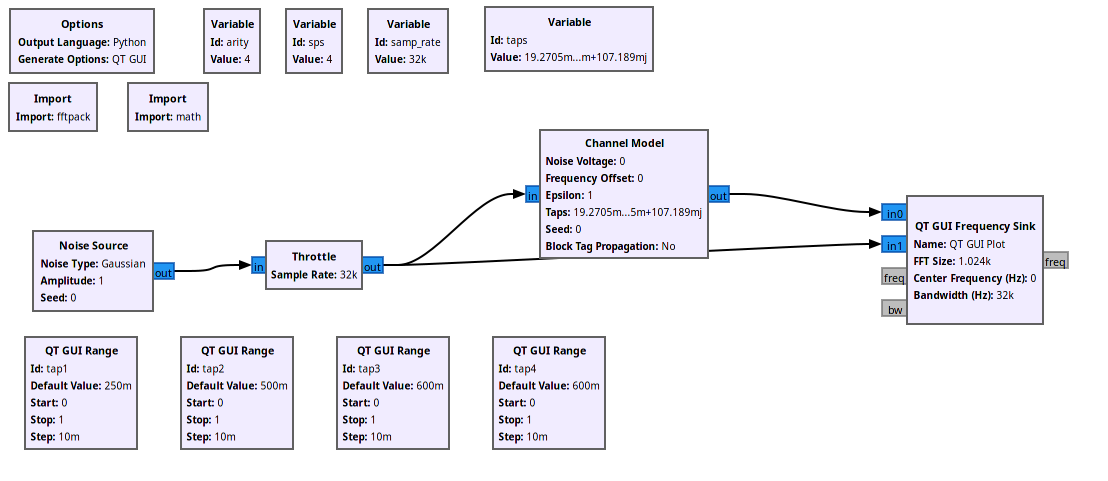
\includegraphics[width=0.75\textwidth]{images/multipath_sim_fg.png}
        \caption{Flow Graph \texttt{multipath\_sim}}
        \label{fig:multipath_sim_fg}
    \end{figure}
    
    В этой симуляции у нас создается канал с 4 управляемыми параметрами, если установить которые в 1, то соответствующие частоты смогут пройти без помех, а при 0 они будут производить \textquote{глубокий нуль} в спектре, что будет влиять так же и на соседние частоты.
    
    Цель в том, чтобы сделать эквалайзер, после работы которого искаженный принятый сигнал бы отражался снова как горизонтальная прямая.
    
    \begin{figure}[H]
        \centering
        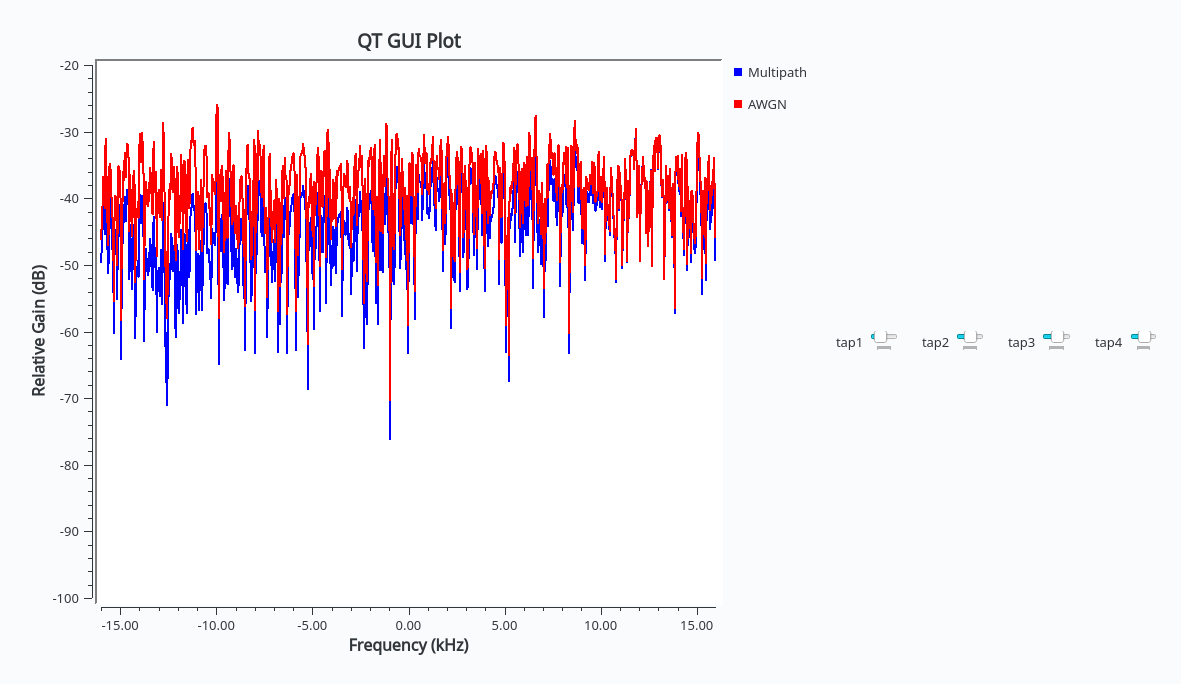
\includegraphics[width=0.75\textwidth]{images/multipath_sim_plot.png}
        \caption{График \texttt{multipath\_sim}}
        \label{fig:multipath_sim_plot}
    \end{figure}
    
    \chapter{Эквалайзеры}
    
    В GNU Radio есть два удобных встроенных эквалайзера: CMA и LMS DD. Constant Modulus Algorithm - это \textquote{слепой} эквалайзер, но он работает лишь с сигналами с постоянной амплитудой, что хорошо работает с цифровыми сигналы вроде MPSK.
    
    Пример ниже демонстрирует MPSK-эквалайзер (параметры подстроены согласно прошлому опыту).
    
    \begin{figure}[H]
        \centering
        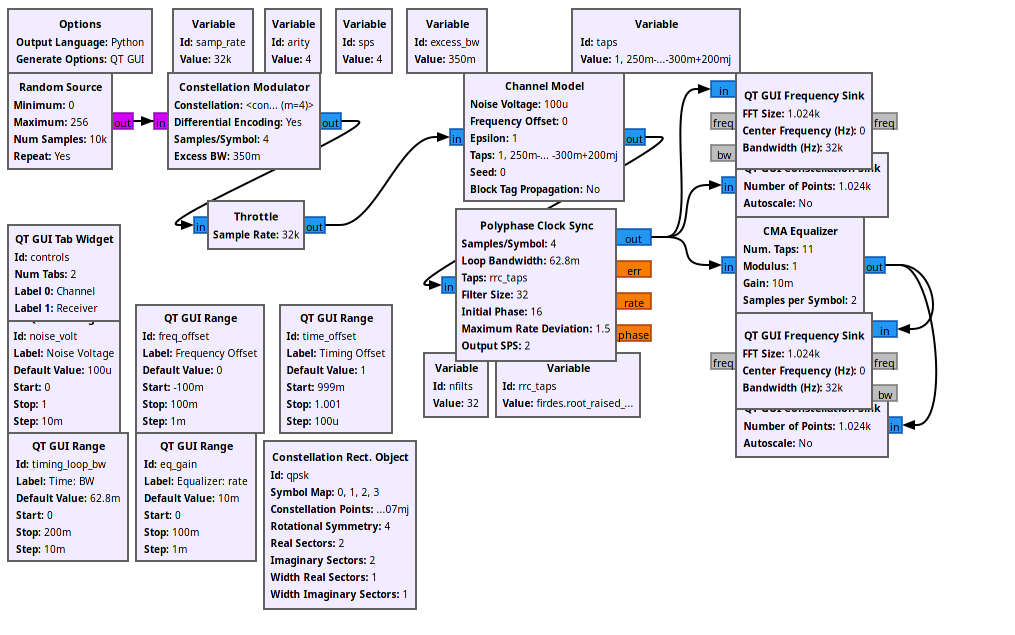
\includegraphics[width=0.75\textwidth]{images/mpsk_stage4_fg.png}
        \caption{Flow Graph \texttt{mpsk\_stage4}}
        \label{fig:mpsk_stage4_fg}
    \end{figure}
    
    Можно видеть, как CMA сходится. У нас тут есть и синхронизация тактирующего сигнала, и блок эквалайзера, и сходятся они независимо, но одна стадия влияет на другую, поэтому некоторое взаимодействие между ними все же есть. В итоге, ниже ы наблюдаем сигнал \textquote{до} и \textquote{после} эквалайзера, и можно видеть, что даже без шума \textquote{до} сигнал выглядит некрасиво, но эквалайзеру удается успешно инвертировать и избавиться от канала.
    
    \begin{figure}[H]
        \centering
        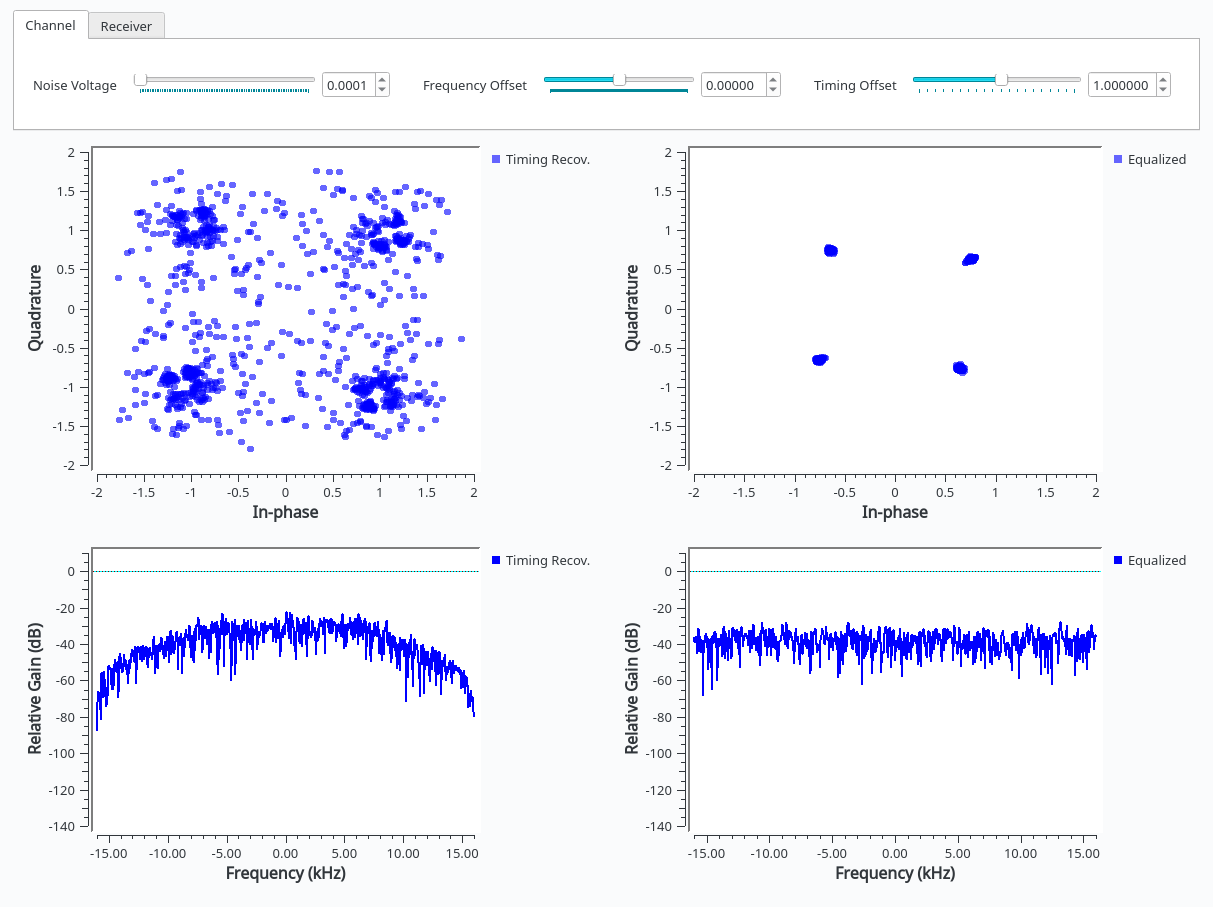
\includegraphics[width=0.75\textwidth]{images/mpsk_stage4_plot.png}
        \caption{График \texttt{mpsk\_stage4}}
        \label{fig:mpsk_stage4_plot}
    \end{figure}
    
    \chapter{LMS-DD Эквалайзер}
    
    Хорошим упражнением было бы попробовать применить Least Mean Squared Decision-Directed эквалайзер. Многие параметры схожи, но есть одно важное отличие от CMA: теперь нам нужна дополнительная информация о принятом сигнале. Эквалайзеру нужно знать точки созвездия.
    
    Этот эквалайзер хорошо подходит для сигналов, которые не подходят под требование постоянной амплитуды (как в CMA), поэтому его можно использовать и для QAM-модуляции. С другой стороны, если все достаточно плохо с SNR, принимаемые эквалайзером решения могут быть некорректными, что заметно снизит производительность приемника. Да и сам блок тоже вычислительно более сложный. Впрочем, если сигнал хороший, то этот эквалайзер может выдать заметно более хороший результат (у него же есть информация о сигнале). Часто сначала используют слепой эквалайзер, когда еще ничего неясно с сигналом, а потом можно переключиться на LMS-DD, но мы не будет так все усложнять.
    
    Заменим CMA на LMS-DD:
    
    \begin{figure}[H]
        \centering
        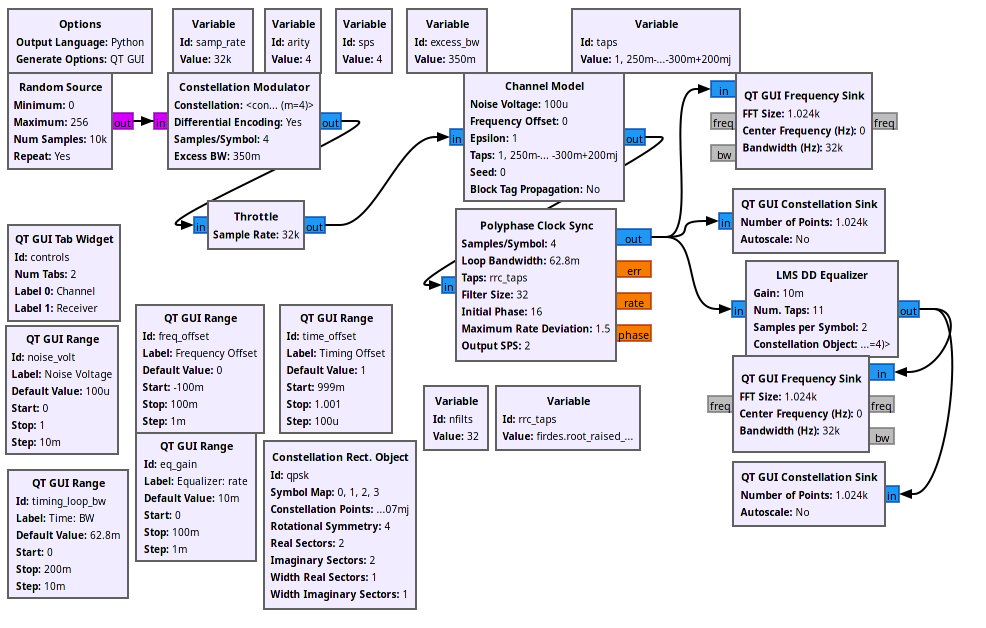
\includegraphics[width=0.75\textwidth]{images/mpsk_stage4_lms_dd_fg.png}
        \caption{Flow Graph \texttt{mpsk\_stage4\_lms\_dd}}
        \label{fig:mpsk_stage4_lms_dd_fg}
    \end{figure}
    
    \begin{figure}[H]
        \centering
        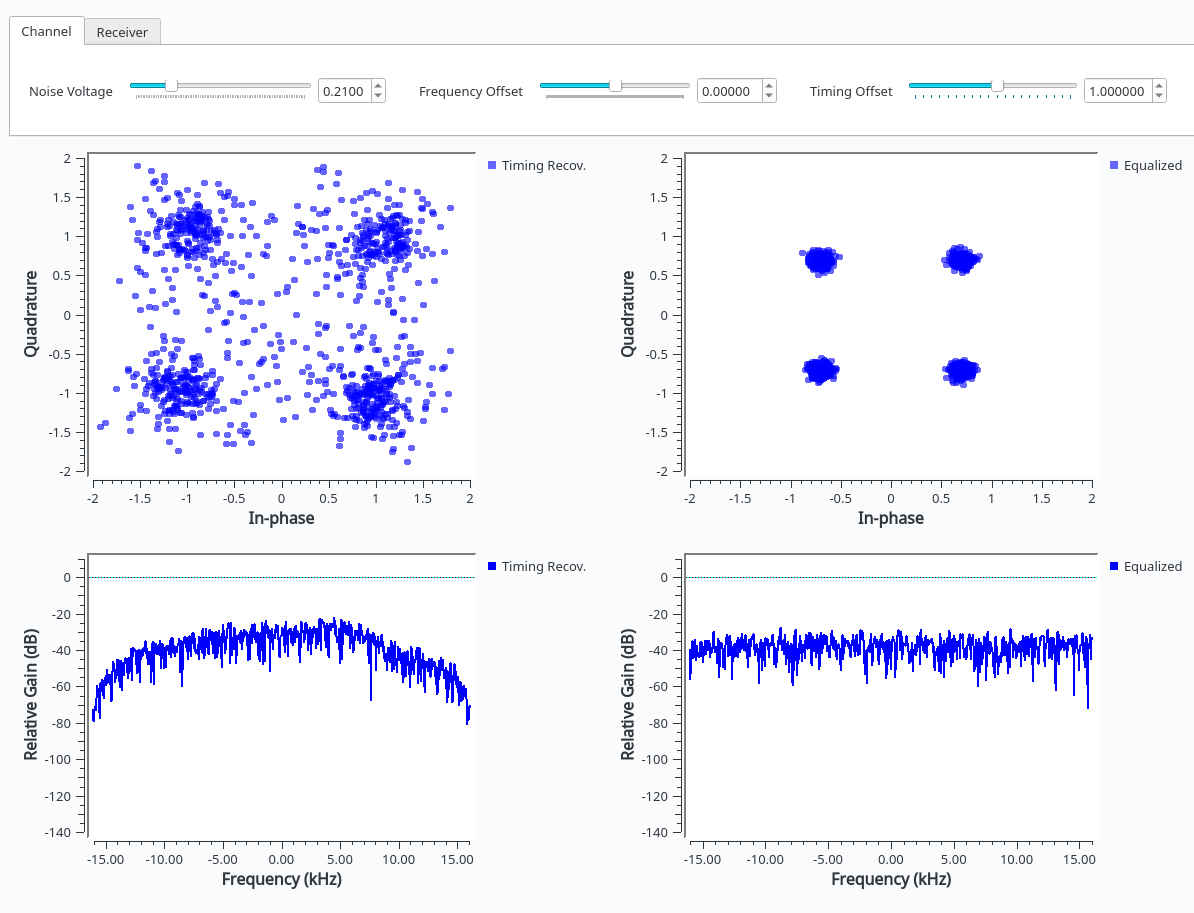
\includegraphics[width=0.75\textwidth]{images/mpsk_stage4_lms_dd_plot.png}
        \caption{График \texttt{mpsk\_stage4\_lms\_dd}}
        \label{fig:mpsk_stage4_lms_dd_plot}
    \end{figure}
    
    \chapter{Подгонка фазы и частоты}
    
    После применения эквалайзера у нас все еще остается проблема со смещением в фазе и частоте. Эквалайзеры часто небыстро адаптируются, так что из-за сдвига частот они могут быстро перестать успевать. К тому же, CMA-эквалайзер ничего не знает о точках созвездия, так что могут возникать проблемы и с тем, какую фазу он начнет использовать как точку отсчета.
    
    Есть два нюанса. Во-первых, мы будем использовать цикл второго порядка, чтобы следить за фазой и частотой с течением времени. Во-вторых, восстановление подразумевает, что мы будем делать \emph{достаточно} хорошую коррекцию частот, поэтому нам нужно будет убедиться, что мы достаточно близки к идеальной частоте. Иначе наш цикл не будет сходиться.
    
    В этом задании мы воспользуемся циклом Костаса. Соответствующий блок может синхронизировать BPSK, QPSK и 8PSK.
    
    \begin{figure}[H]
        \centering
        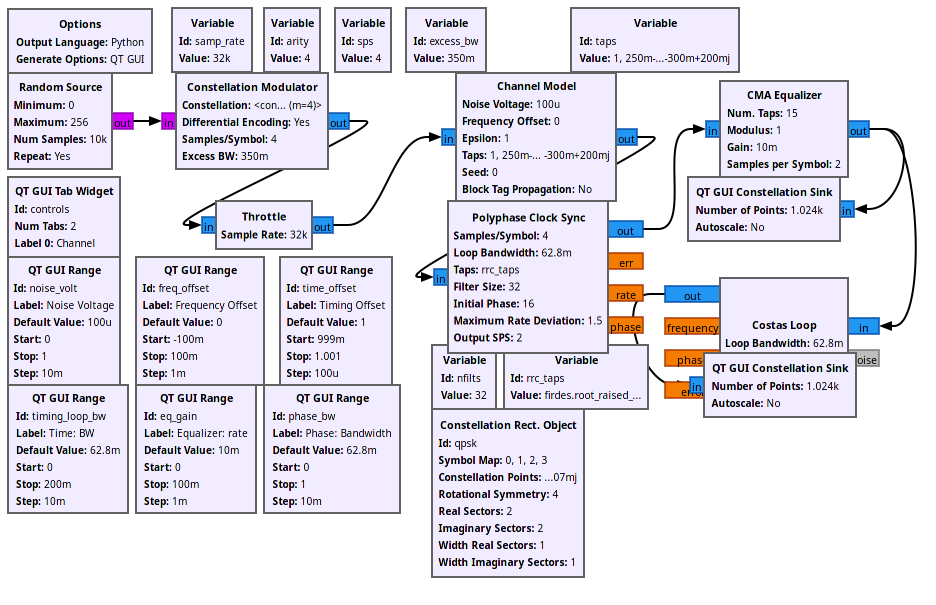
\includegraphics[width=0.75\textwidth]{images/mpsk_stage5_fg.png}
        \caption{Flow Graph \texttt{mpsk\_stage5}}
        \label{fig:mpsk_stage5_fg}
    \end{figure}
    
    Этот блок, как и все наши другие, использует цикл второго порядка, а потому и имеет соответствующий параметр, связанный с пропускной способностью. Ему также нужно знать степень PSK-модуляции (4 для QPSK). Можно видеть, как после работы эквалайзера все символы расположены на единичной окружности, но из-за сдвига частот, они как бы \textquote{размазаны} по ней, а не соответствуют нашим 4 точкам. После цикла Костаса мы уже видим ровно 4 исходные точки, но некоторый шум тоже присутствует.
    
    \begin{figure}[H]
        \centering
        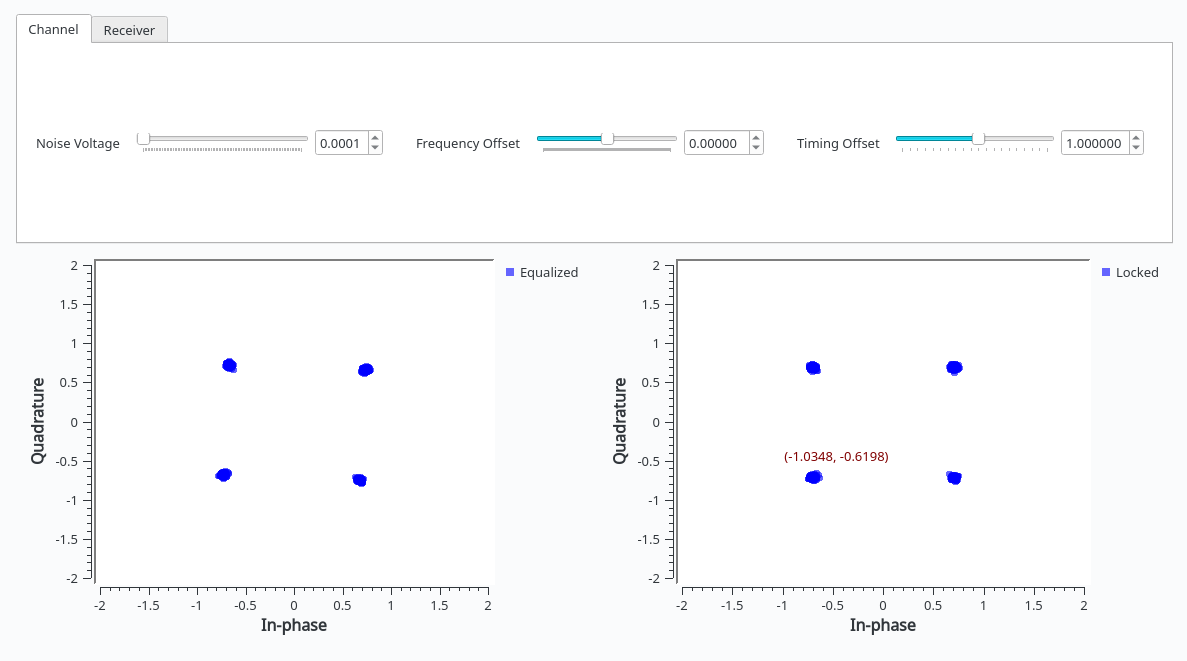
\includegraphics[width=0.75\textwidth]{images/mpsk_stage5_plot.png}
        \caption{График \texttt{mpsk\_stage5}}
        \label{fig:mpsk_stage5_plot}
    \end{figure}
    
    \chapter{Декодер}
    
    Теперь, когда сложная часть пройдена, можно делать декодер. После цикла Костаса мы вставляем еще \sloppy{\texttt{Constellation Decoder}}, но это еще не все. На этом этапе мы видим символы 0..3, потому что на это рассчитан наш алфавит, но у нас нет никакой уверенности, что эти 0..3 правильно соответствуют тем 0..3, что мы передавали изначально. Нам удавалось обходить этот вопрос, потому что мы использовали дифференциальное кодирование в \sloppy{\texttt{Constellation Modulator}}'е. Выключим теперь это.
    
    \begin{figure}[H]
        \centering
        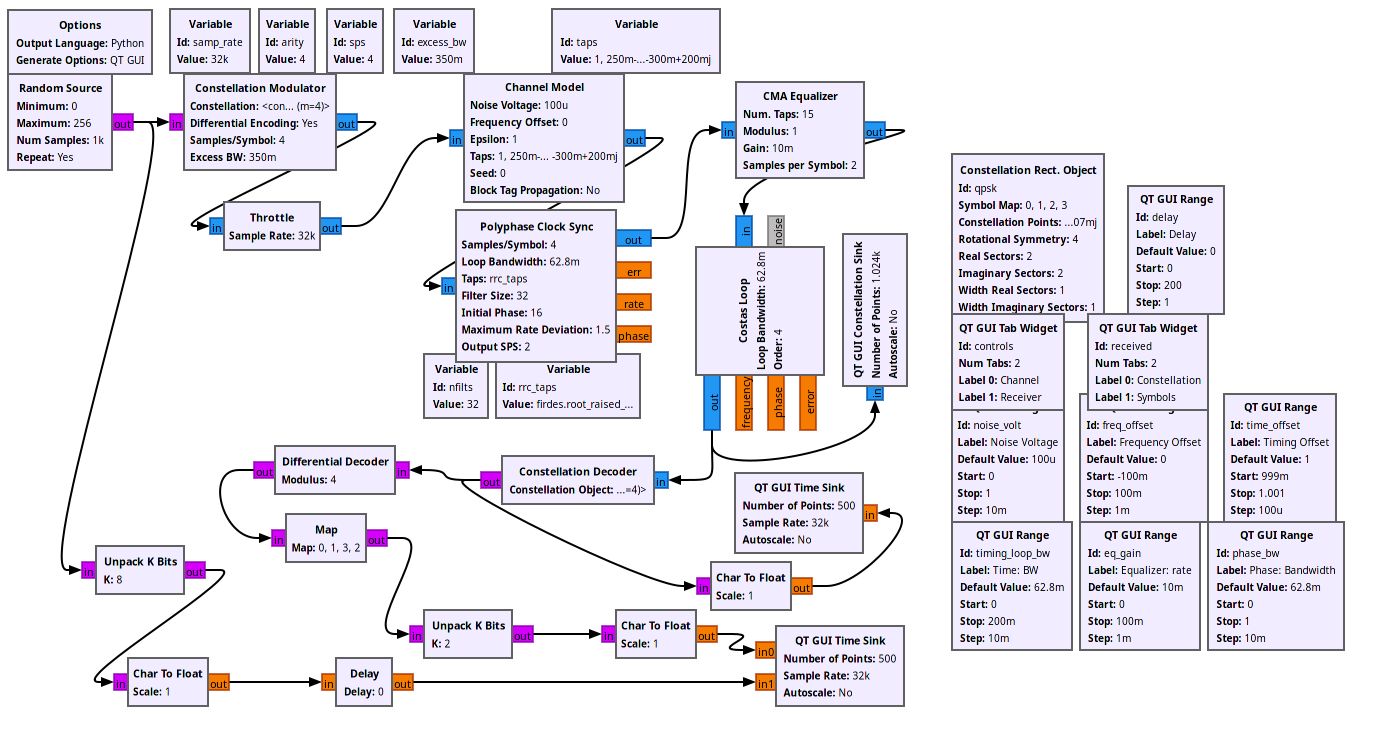
\includegraphics[width=0.75\textwidth]{images/mpsk_stage6_fg.png}
        \caption{Flow Graph \texttt{mpsk\_stage6}}
        \label{fig:mpsk_stage6_fg}
    \end{figure}
    
    Flow Graph использует блок \sloppy{\texttt{Differential Decoder}}, чтобы перевести дифференциально-закодированные символы обратно в исходные при помощи сдвигов фаз, а не абсолютной фазы. Но даже так наши символы еще не совсем верные. Во время синхронизации математика и физика была на нашей стороне, а теперь нам надо интерпретировать символы, основываясь на том, что кто-т осказал, какими они были. То есть, нам просто надо знать, как они соотносятся. Для этого мы воспользуемся блоками \sloppy{\texttt{Map}} и \sloppy{\texttt{Unpack Bit}}.
    
    Чтобы убедиться, что теперь мы действительно получаем \emph{тот самый поток данных}, мы просто сравним, что было в начале, с тем, что получили (ведь это симуляция, мы имеем доступ к любой информации). Передатчик создает упакованные биты, поэтому при помощи \sloppy{\texttt{Unpack Bit}} мы должны их распаковать из 8 бит на байт в 1 бит на байт, затем превратить их в \sloppy{\texttt{float}} 0.0 и 1.0, потому что \sloppy{\texttt{Time Sink}} умеет только \sloppy{\texttt{float}} и \sloppy{\texttt{complex}} принимать. Но напрямую сравнивать значения пока нельзя, потому что в приемнике есть еще много узлов, которые задерживают данные, поэтому нам нужен еще и блок \sloppy{\texttt{Delay}}.
    
    \begin{figure}[H]
        \centering
        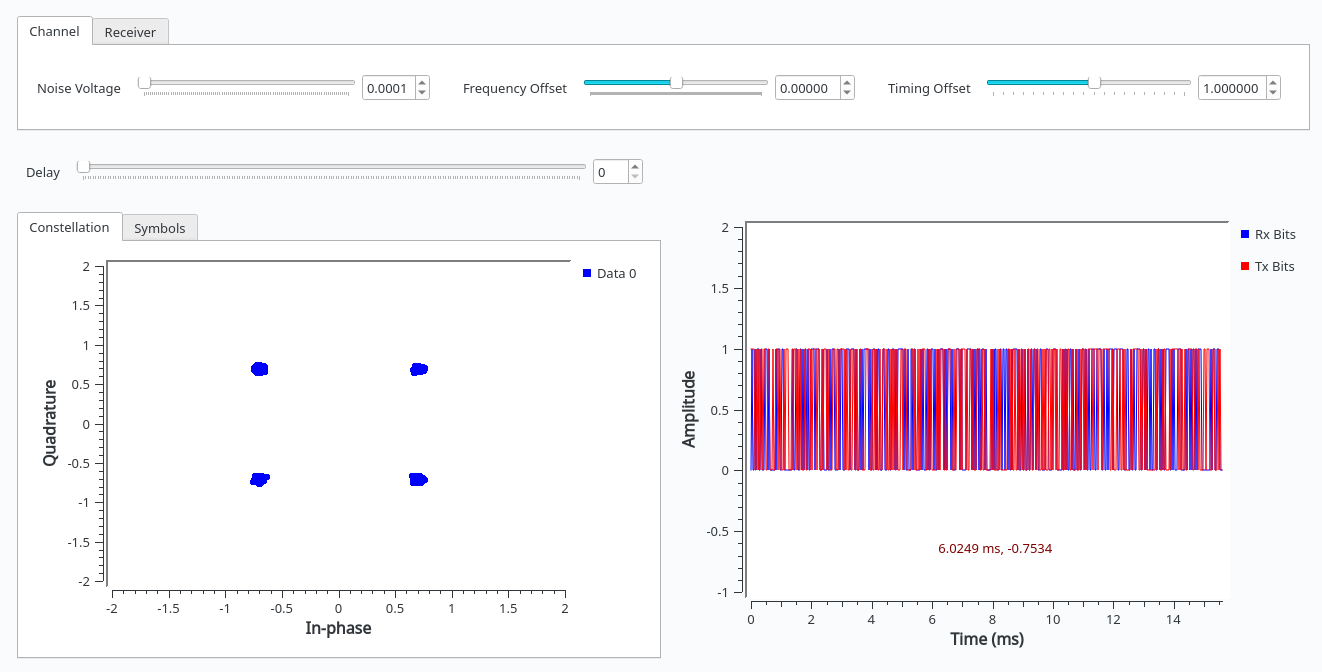
\includegraphics[width=0.75\textwidth]{images/mpsk_stage6_plot.png}
        \caption{График \texttt{mpsk\_stage6}}
        \label{fig:mpsk_stage6_plot}
    \end{figure}
    
    \chapter{Выводы}
    
    В процессе выполнения работы мы разобрались с тем, как произвести установку и настройку GNU Radio, а также рассмотрели множество явлений, связанныйх с передачей QPSK-сигнала. Симулируя настоящие условия передачи данных, мы столкнулись с рядом возможных трудностей, а также рассмотрели и пути их решения, что поможет нам в будущем при организации настоящих каналов передач.

    \printbibliography
    
\end{document}
